% Estrutura adaptada do template institucional fornecido.
\documentclass[12pt,a4paper,twoside]{article}
\usepackage[left=3cm,top=3cm,right=2cm,bottom=2cm]{geometry}
\usepackage[T1]{fontenc}
\usepackage[brazilian]{babel}
\usepackage{amsmath,amssymb,bm}
\usepackage{graphicx,booktabs,array,longtable}
\usepackage{fancyhdr,titletoc,titlesec,setspace,indentfirst}
\usepackage{caption,float,placeins}
\usepackage[colorlinks=true,allcolors=black,bookmarksnumbered=true]{hyperref}
\usepackage{bookmark}
\usepackage[alf]{abntex2cite}
\numberwithin{equation}{section}
\newcommand{\titulo}{Contribuição preditiva de representações de letras para a popularidade no Spotify}
\newcommand{\autor}{Felipe Macedo Cordeiro}
\newcommand{\orientador}{Leandro Tavares Correia}
\newcommand{\fonte}[1]{\par\vspace{2pt}{\footnotesize Fonte: #1\par}}
\newcommand{\nota}[1]{\par\vspace{2pt}{\footnotesize #1\par}}
\newcommand{\notafigura}[1]{\if\relax\detokenize{#1}\relax\else\nota{#1}\fi}
\newcommand{\figura}[5][.42\textheight]{%
  \begin{figure}[!htbp]\centering
  \caption{#3}\label{#4}%
  \includegraphics[width=\linewidth,height=#1,keepaspectratio]{images/#2.png}%
  \notafigura{#5}%
  \end{figure}}
\setcounter{topnumber}{3}
\setcounter{bottomnumber}{2}
\setcounter{totalnumber}{4}
\renewcommand{\topfraction}{.87}
\renewcommand{\bottomfraction}{.74}
\renewcommand{\textfraction}{.10}
\renewcommand{\floatpagefraction}{.71}
\newcolumntype{P}[1]{>{\raggedright\arraybackslash}p{#1}}
\pagestyle{fancy}\fancyhf{}
\setlength{\headheight}{16pt}
\fancyhead[RO,LE]{\thepage}
\fancyhead[RE,LO]{\nouppercase{\emph{\leftmark}}}
\renewcommand{\sectionmark}[1]{\markboth{#1}{}}
\titlecontents{section}[0cm]{}{\bfseries\thecontentslabel\ }{}{\titlerule*[.75pc]{.}\contentspage}
\titlecontents{subsection}[.75cm]{}{\thecontentslabel\ }{}{\titlerule*[.75pc]{.}\contentspage}
\setcounter{secnumdepth}{3}\setcounter{tocdepth}{2}
\captionsetup{font=small,labelfont=normalfont,justification=centering}
\setlength{\parindent}{1.5cm}\setlength{\parskip}{0.15cm}
\setlength{\intextsep}{9pt plus 2pt minus 2pt}
\setlength{\textfloatsep}{12pt plus 3pt minus 3pt}
\setlength{\floatsep}{9pt plus 2pt minus 2pt}
\titlespacing*{\section}{0cm}{0cm}{0.5cm}
\titlespacing*{\subsection}{0cm}{0.43cm}{0.22cm}
\raggedbottom
\hypersetup{pdftitle={Contribuição preditiva de representações de letras para a popularidade no Spotify},pdfauthor={Felipe Macedo Cordeiro}}
\begin{document}
\hypersetup{pageanchor=false}
\begin{titlepage}
\centering

\includegraphics[scale=.8]{imagens/unb.png}\par
\vspace{.4cm}
\textbf{Universidade de Brasília\\Departamento de Estatística}\par
\vspace{4.2cm}
\textbf{\titulo}\par
\vspace{2cm}
\textbf{\autor}\par
\vspace{1.5cm}
\begin{flushright}
\begin{minipage}{7.5cm}
Relatório apresentado ao Departamento de Estatística da Universidade de Brasília como parte dos requisitos necessários para obtenção do grau de Bacharel em Estatística.
\end{minipage}
\end{flushright}
\vfill
\textbf{Brasília\\2026}
\end{titlepage}

\thispagestyle{empty}
\begin{center}
\textbf{\autor}\par
\vspace{4cm}
\textbf{\titulo}\par
\vspace{2cm}
Orientador: \orientador
\end{center}
\vspace{2cm}
\begin{flushright}
\begin{minipage}{7.5cm}
Relatório apresentado ao Departamento de Estatística da Universidade de Brasília como parte dos requisitos necessários para obtenção do grau de Bacharel em Estatística.
\end{minipage}
\end{flushright}
\vfill
\begin{center}\textbf{Brasília\\2026}\end{center}

\clearpage\pagenumbering{gobble}
\onehalfspacing
\thispagestyle{empty}
\vspace*{2.5cm}
\begin{center}
{\Huge\bfseries Resumo}
\end{center}
\vspace{1.5cm}
\begin{spacing}{1.35}
Este trabalho avalia quanto as letras acrescentam à classificação da popularidade musical quando já se conhecem atributos acústicos e metadados. A partir de um catálogo de 1.159.764 faixas do Spotify, dimensionou-se um sorteio estratificado de 9.526 faixas. A consulta ao LRCLIB recuperou letras para 3.869 das faixas sorteadas. Em um quadro consolidado de 80.943 vínculos aceitos, selecionou-se uma coorte de modelagem com 9.526 faixas, todas com letra. Os escores observados foram agrupados em três níveis, baixo (0--19), médio (20--39) e alto (40--100). Compararam-se quatro regressões logísticas ordinais penalizadas em validação cruzada aninhada por grupos. As acurácias balanceadas foram 56,14\% com áudio e metadados, 56,24\% com a adição de descritores lexicais, 55,91\% com a adição de embeddings e 55,96\% com a inclusão de ambas as representações. Com embeddings, a sensibilidade da classe alta subiu de 26,25\% para 31,07\% no modelo Profundo, acompanhada de menor precisão nessa classe. O bootstrap condicionado às previsões incluiu zero nos contrastes de acurácia balanceada. Os resultados indicam ganho global limitado e redistribuição de erros nas faixas com letra analisadas.
\end{spacing}

\vspace{1.5cm}
\noindent Palavras-chave: popularidade musical, letras de músicas, amostragem estratificada, regressão ordinal, representações textuais.


\clearpage
\begingroup\small\singlespacing
\listoftables
\clearpage
\listoffigures
\endgroup
\clearpage\tableofcontents
\clearpage\pagenumbering{arabic}\hypersetup{pageanchor=true}
\section{Introdução}\label{sec:introducao}
Uma mesma faixa pode ser descrita pelo som, pelo contexto de lançamento e pelo conteúdo da letra. Essas fontes de informação podem ser parcialmente redundantes. Gênero e atributos acústicos, por exemplo, já descrevem aspectos do estilo musical que também aparecem no texto. A questão deste trabalho é se conhecer a letra melhora a classificação do nível de popularidade observado no Spotify quando áudio e metadados já estão disponíveis.

\citeonline{dhanaraj2005} investigaram a combinação de texto e áudio na classificação de sucesso musical. \citeonline{singhi2014} estudaram características de letras para distinguir músicas populares. Já \citeonline{parada2024lyrics} analisaram a contribuição textual em dados de escuta da Last.fm. A comparação direta dos desempenhos exige atenção às respostas de cada estudo. Neste trabalho, a resposta é o escore fornecido pelo Spotify no arquivo disponível. Para a análise, ele é dividido em três níveis ordenados.

O objetivo é medir a contribuição incremental de dois tipos de representação das letras, descritores lexicais e estruturais e embeddings multilíngues. A comparação usa quatro configurações ajustadas nas mesmas faixas e divisões, com o mesmo modelo estatístico. Examina-se tanto o desempenho médio entre classes quanto o tipo de erro que passa a ocorrer com cada representação. O desempenho refere-se à classificação do escore observado, sem um horizonte futuro de previsão.

A integração segue quatro passos. Primeiro, descrevem-se o catálogo acessível do Spotify e a estrutura da base LRCLIB. Depois, dimensiona-se e sorteia-se uma amostra probabilística do catálogo para orientar a recuperação e aferir sua cobertura. Em seguida, os vínculos aceitos dessa busca e de buscas anteriores são reunidos em um quadro com letras. Dele saem as 9.526 faixas usadas pelos quatro classificadores. A distinção entre o sorteio inicial e a seleção no quadro vinculado determina quais resultados podem ser atribuídos ao catálogo acessível e quais descrevem a coorte de modelagem.


\section{Fontes e análise descritiva}\label{sec:fontes}
\subsection{Catálogo Spotify e qualidade dos campos}
O arquivo público disponibilizado no Kaggle por \texttt{amitanshjoshi} sob o nome \textit{Spotify\_1Million\_Tracks} contém 1.159.764 linhas, com identificadores Spotify distintos, e 20 campos \cite{spotifydataset}. Essa é a população finita acessível. A fonte não documenta um desenho de seleção a partir da plataforma inteira. Cada linha é uma faixa, de modo que versões ou gravações de uma composição podem ter IDs diferentes. Há 64.157 créditos de artista distintos como cadeias de caracteres, 882.360 títulos distintos, 15 créditos ausentes e um título ausente. Os campos de identificação não servem como preditores. A Tabela~\ref{tab:dicionario} apresenta o dicionário.

\begingroup\footnotesize\singlespacing
\begin{longtable}{@{}P{.26\linewidth}P{.20\linewidth}P{.48\linewidth}@{}}
\caption{Dicionário dos campos do arquivo Spotify.}\label{tab:dicionario}\\
\toprule Campo & Tipo ou unidade & Definição operacional \\\midrule\endfirsthead
\toprule Campo & Tipo ou unidade & Definição operacional \\\midrule\endhead
\bottomrule\endfoot
\bottomrule\endlastfoot
Sem nome & Índice & Índice exportado no CSV. \\
\texttt{track\_id} & Texto & Identificador da faixa Spotify. \\
\texttt{track\_name} & Texto & Título informado. \\
\texttt{artist\_name} & Texto & Crédito de artista informado. \\
\texttt{popularity} & Inteiro 0--100 & Escore observado de popularidade. \\
\texttt{year} & Ano inteiro & Ano informado na fonte. \\
\texttt{genre} & Categoria & Rótulo de gênero fornecido. \\
\texttt{danceability} & Escore 0--1 & Adequação estimada à dança. \\
\texttt{energy} & Escore 0--1 & Intensidade e atividade percebidas. \\
\texttt{key} & Classe 0--11 & Classe de altura musical, com $-1$ se não identificada. \\
\texttt{loudness} & Decibéis (dB) & Intensidade sonora média informada. \\
\texttt{mode} & Categoria 0/1 & Modo menor ou maior. \\
\texttt{speechiness} & Escore 0--1 & Presença estimada de fala. \\
\texttt{acousticness} & Escore 0--1 & Grau estimado de caráter acústico. \\
\texttt{instrumentalness} & Escore 0--1 & Estimativa de ausência de voz. \\
\texttt{liveness} & Escore 0--1 & Indícios de execução ao vivo. \\
\texttt{valence} & Escore 0--1 & Positividade musical estimada. \\
\texttt{tempo} & BPM & Andamento global estimado. \\
\texttt{duration\_ms} & Milissegundos & Duração da faixa. \\
\texttt{time\_signature} & Categoria & Assinatura de tempo estimada. \\
\end{longtable}
\fonte{Arquivo Spotify\_1Million\_Tracks \cite{spotifydataset} e documentação do Spotify \cite{spotifyaudio,spotifydocs}.}
\endgroup



A popularidade é um escore de zero a cem. A documentação da plataforma associa a medida ao volume e à recência de reproduções \cite{spotifydocs}. A data de medição do escore no arquivo e a versão exata do CSV não foram confirmadas. O ano registrado é usado como metadado fornecido, pois a fonte não permite assegurar que seja o primeiro lançamento da composição. Os atributos acústicos também são fornecidos no arquivo e não foram extraídos novamente do áudio \cite{spotifyaudio}.

\subsection{Distribuições marginais e período}
A popularidade tem média de 18,38, mediana de 15 e percentil 95 de 49. Há 158.391 faixas com escore zero (13,66\%) e 499 com escore entre 80 e 100 (0,043\%). A transformação $\log(1+s)$, para escore $s$, preserva os zeros. Na Figura~\ref{fig:poplog}, ela inverte o sentido da assimetria de $0,810$ para $-0,795$, com pouca mudança em magnitude. O modelo final utiliza os limites na escala original.

\figura[.24\textheight]{02_popularidade_original_log1p}{Distribuição da popularidade nas escalas original e logarítmica.}{fig:poplog}{A escala logarítmica usa $\log(1+s)$.}

O ano informado concentra 443.801 faixas em 2000--2009, 514.990 em 2010--2019 e 200.973 em 2020--2023 (Figura~\ref{fig:anos}). As popularidades médias nesses três grupos são 12,66, 19,99 e 26,89, respectivamente. Essa associação pode refletir a composição da fonte e a relação entre recência e escore. A presença de uma observação por faixa impede acompanhar a evolução individual ao longo do tempo.

\figura[.24\textheight]{04_anos}{Número de faixas por ano informado no catálogo.}{fig:anos}{}

A Tabela~\ref{tab:numericos} resume os atributos numéricos. A instrumentalidade tem mediana de 0,00176 e terceiro quartil de 0,614, ilustrando a grande diferença entre partes da distribuição. As distribuições de presença de fala e de indício de execução ao vivo têm caudas à direita. Dançabilidade se concentra em valores intermediários e energia tem maior presença em escores altos. A duração mediana é 225,74 segundos, com 448,00 segundos no percentil 95 e máximo de aproximadamente 100 minutos. O histograma de amplitude completa torna essa cauda visível. Os quantis caracterizam a região típica com maior resolução.

\begin{table}[H]\centering\footnotesize
\caption{Resumo das variáveis numéricas no catálogo.}\label{tab:numericos}
\setlength{\tabcolsep}{4.0pt}
\begin{tabular}{@{}lrrrrrr@{}}\toprule
Variável & Média & DP & P25 & Mediana & P75 & P95 \\\midrule
Popularidade & 18,38 & 15,89 & 5,00 & 15,00 & 29,00 & 49,00 \\
Ano informado & 2011,96 & 6,80 & 2006,00 & 2012,00 & 2018,00 & 2022,00 \\
Dançabilidade & 0,5374 & 0,1845 & 0,4130 & 0,5500 & 0,6770 & 0,8110 \\
Energia & 0,6397 & 0,2705 & 0,4540 & 0,6940 & 0,8730 & 0,9760 \\
Intensidade sonora (dB) & -8,98 & 5,68 & -10,83 & -7,45 & -5,28 & -3,15 \\
Presença de fala & 0,0928 & 0,1268 & 0,0371 & 0,0507 & 0,0890 & 0,2980 \\
Caráter acústico & 0,3215 & 0,3550 & 0,0064 & 0,1470 & 0,6400 & 0,9760 \\
Instrumentalidade & 0,2523 & 0,3651 & 0,0000 & 0,0018 & 0,6140 & 0,9230 \\
Vivacidade & 0,2230 & 0,2011 & 0,0979 & 0,1340 & 0,2920 & 0,7080 \\
Valência & 0,4556 & 0,2685 & 0,2260 & 0,4380 & 0,6740 & 0,9100 \\
Andamento (BPM) & 121,38 & 29,78 & 98,80 & 121,93 & 139,90 & 174,88 \\
Duração (s) & 249,56 & 149,43 & 181,09 & 225,74 & 286,91 & 448,00 \\
\bottomrule
\end{tabular}\nota{$N=1.159.764$ por variável. O DP usa divisor $N$. Andamento inclui zeros.}
\end{table}


Há 1.199 faixas com andamento zero, das quais 650 pertencem ao gênero \textit{sleep}. Os registros foram preservados no catálogo e nos momentos do dimensionamento. A descrição gráfica de andamento e as análises de correlação e PCA usam a regra de andamento positivo. O tratamento separa explicitamente esses denominadores. Os campos numéricos de áudio e duração aparecem na Figura~\ref{fig:distacustica}.

As categorias musicais também exibem concentração. O modo maior corresponde a 63,47\% das faixas. A assinatura de tempo codificada como 4 responde por 87,14\%. Na tonalidade, as classes mais frequentes são 7 (12,04\%) e 0 (11,22\%). Essas variáveis são tratadas como categorias na modelagem. A Figura~\ref{fig:categoriasmusicais} apresenta a distribuição completa de seus níveis.

\figura[.54\textheight]{01_distribuicoes_metadados}{Distribuições dos dez atributos acústicos e de duração.}{fig:distacustica}{Cada painel informa o número de valores válidos.}
\figura[.23\textheight]{05_categorias_musicais}{Tonalidade, modo e assinatura de tempo no catálogo.}{fig:categoriasmusicais}{}

\subsection{Gênero e perfis acústicos}
O catálogo tem 82 rótulos de gênero. \textit{Black-metal} é o mais frequente, com 21.852 faixas (1,88\%). \textit{Songwriter} reúne 589 (0,05\%). Os rótulos são mantidos como no arquivo e incluem estilos, usos ou contextos de escuta. As frequências caracterizam a fonte, que não mede participações de mercado. A Figura~\ref{fig:generos} mostra os vinte rótulos mais frequentes.

\figura[.35\textheight]{03_generos}{Vinte rótulos de gênero mais frequentes no catálogo.}{fig:generos}{A tabela de frequências que acompanha o projeto inclui os 82 rótulos.}

Para uma variável $z$ com média $\bar z$, a fração de variação associada às diferenças entre $G$ médias de grupos é
\begin{equation}
\eta^2=\frac{\sum_{g=1}^G N_g(\bar z_g-\bar z)^2}{\sum_i(z_i-\bar z)^2},
\end{equation}
com $N_g$ igual ao número de valores válidos do grupo $g$. Assim, 51,76\% da soma de quadrados de caráter acústico corresponde a diferenças entre gêneros. Para presença de fala, intensidade sonora, energia, dançabilidade, popularidade, instrumentalidade e andamento válido, as frações são 49,96\%, 48,39\%, 45,99\%, 41,86\%, 41,27\%, 40,10\% e 8,50\%, respectivamente. A energia média varia de 0,222 em \textit{classical} a 0,933 em \textit{death-metal}. Isso sustenta a estratificação do sorteio por gênero e indica a necessidade de conferir atributos que variam substancialmente dentro dos gêneros.

As Figuras~\ref{fig:perfis_a} e~\ref{fig:perfis_b} mostram os 82 perfis. Cada célula é a diferença entre a média do gênero e a média do catálogo, expressa em desvios-padrão do campo. O contraste entre energia, intensidade sonora e caráter acústico aparece em vários rótulos. Na Figura~\ref{fig:boxgenres}, os intervalos entre quantis evidenciam a heterogeneidade dentro dos próprios gêneros.

\begin{figure}[!htbp]
\centering
\begin{minipage}[t]{.485\linewidth}
\centering
\caption{Perfis padronizados dos gêneros 1 a 41 em ordem alfabética.}
\label{fig:perfis_a}
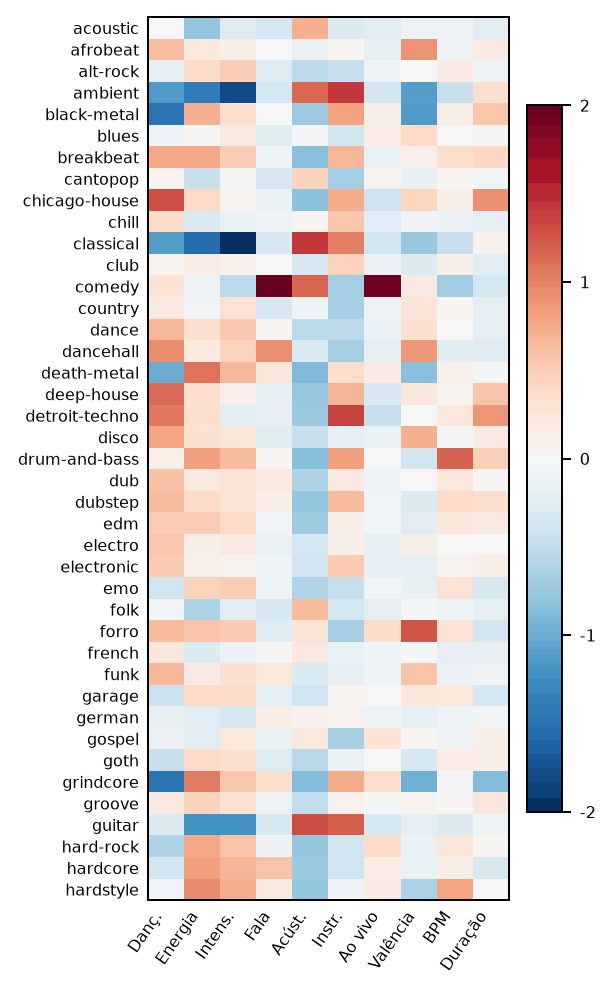
\includegraphics[width=\linewidth]{images/perfil_generos_1.png}
\end{minipage}\hfill%
\begin{minipage}[t]{.485\linewidth}
\centering
\caption{Perfis padronizados dos gêneros 42 a 82 em ordem alfabética.}
\label{fig:perfis_b}
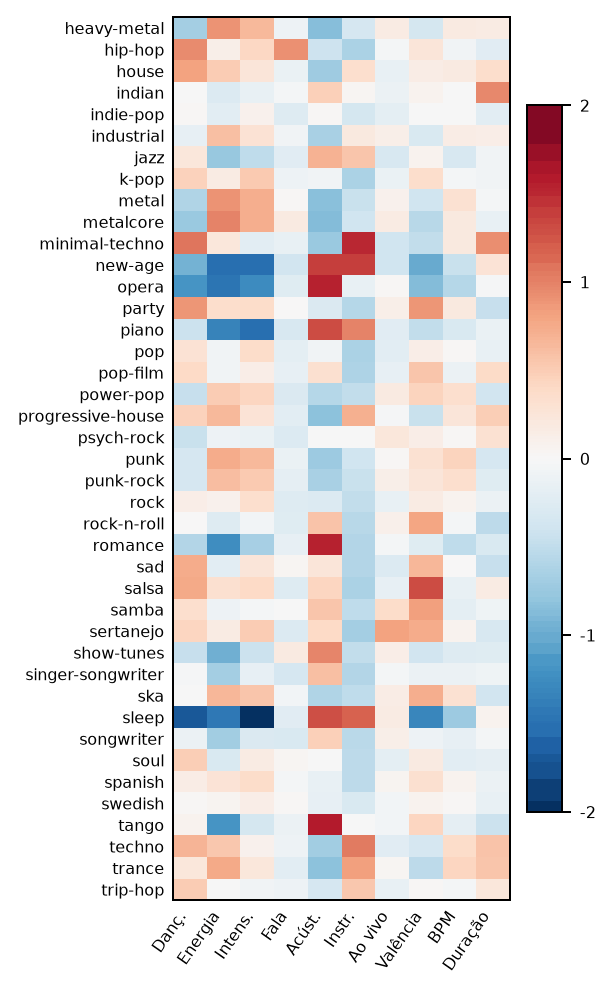
\includegraphics[width=\linewidth]{images/perfil_generos_2.png}
\end{minipage}
\nota{Escala comum em desvios-padrão. Danç. = dançabilidade, Intens. = intensidade
sonora, Acúst. = caráter acústico e Instr. = instrumentalidade.}
\end{figure}

Entre os exemplos do segundo painel, \textit{sleep} tem andamento válido médio de aproximadamente 100 BPM. Em \textit{drum-and-bass}, no primeiro painel, a média é de 157 BPM. Já a instrumentalidade média é de 0,0025 em \textit{sertanejo} e 0,767 em \textit{ambient}. O padrão por gênero é útil para o desenho amostral e para interpretar a perda de cobertura quando um gênero tem poucas faixas vinculadas.

\figura[.49\textheight]{09_distribuicoes_por_genero}{Atributos selecionados nos dez gêneros mais frequentes.}{fig:boxgenres}{Hastes nos percentis 5 e 95, caixas entre os quartis e traço na mediana.}

No agrupamento por período, as diferenças entre médias representam menos de 1\% da variação de cada atributo acústico ou de duração. Para a popularidade, a fração é 10,39\%. Na Figura~\ref{fig:perfilperiodos}, a escala padronizada é a mesma usada na comparação entre gêneros. Os contrastes menores entre períodos são coerentes com os valores de $\eta^2$.

\figura[.25\textheight]{08_perfis_periodos}{Perfis acústicos médios por período, em escala padronizada.}{fig:perfilperiodos}{Diferenças medidas em desvios-padrão em relação ao catálogo.}

\subsection{Associações entre atributos e componentes principais}
O conjunto de casos completos para as análises bivariadas reúne 1.158.565 faixas. A Figura~\ref{fig:corr} apresenta as correlações de Pearson e Spearman nas mesmas observações. Por Pearson, energia tem correlação de 0,781 com intensidade sonora e de $-0,754$ com caráter acústico. Dançabilidade e valência têm correlação de 0,518. As direções principais se mantêm nas correlações de postos. As densidades da Figura~\ref{fig:densidades} mostram concentrações e variações conjuntas que um único coeficiente não resume.

\figura[.30\textheight]{06_correlacoes}{Correlações de Pearson e de Spearman no catálogo.}{fig:corr}{Análise de casos completos válidos.}

As duas matrizes concordam quanto aos principais sinais. A correlação entre caráter acústico e intensidade sonora, por exemplo, é $-0,623$ pela medida de Pearson e $-0,566$ pela de Spearman. A densidade dos pares ajuda a interpretar esses coeficientes porque as faixas não ocupam a escala de forma uniforme. No caso da instrumentalidade, a acumulação perto de zero faz parte dessa estrutura.

\figura[.47\textheight]{10_relacoes_metadados}{Densidades de pares de atributos no catálogo.}{fig:densidades}{Frequências por célula nos pares indicados.}

A análise de componentes principais (PCA) usa as dez colunas numéricas de áudio e duração. Cada uma é centrada pela média e dividida pelo desvio-padrão amostral. Para a matriz padronizada $Z$, com $m$ faixas, os autovetores unitários $v_j$ de $Z^\top Z/(m-1)$ são ordenados segundo os autovalores $\lambda_j$, do maior para o menor. O componente tem escores $Zv_j$ e explica a fração $\lambda_j/\sum_\ell\lambda_\ell$ da variância padronizada \cite{jolliffe2002,jolliffe2016}. Popularidade, ano e categorias permanecem fora dos eixos.

O primeiro componente explica 29,12\%; os dois primeiros, 44,35\%; e os três, 57,85\%. São necessários seis para 84,39\% e oito para 95,66\% (Figura~\ref{fig:pca_var}). O primeiro eixo contrapõe energia e intensidade sonora a caráter acústico. O segundo associa valência e dançabilidade na direção oposta a instrumentalidade e duração. Presença de fala e indício de execução ao vivo destacam-se no terceiro eixo. Os coeficientes dos autovetores estão na Figura~\ref{fig:pca_coef}. O sinal de cada eixo é convencional.

\figura[.24\textheight]{11_pca_variancia}{Variância padronizada explicada pelos componentes principais.}{fig:pca_var}{Frações por componente e acumuladas.}
\figura[.30\textheight]{12_pca_coeficientes}{Coeficientes dos autovetores nos três primeiros componentes.}{fig:pca_coef}{}

Os eixos revelam redundância parcial, mas a projeção dos dois primeiros descarta mais da metade da variância dos preditores (Figura~\ref{fig:pca_mapa}). A PCA foi usada para caracterizar os metadados. O Baseline conserva os atributos originais e a regularização controla a complexidade do ajuste.

\figura[.30\textheight]{13_pca_mapa}{Densidade de faixas no plano dos dois primeiros componentes.}{fig:pca_mapa}{}
\FloatBarrier

\subsection{LRCLIB e estrutura dos registros}
O LRCLIB é um repositório aberto de letras, alimentado por contribuições. A base utilizada corresponde ao dump público de 12 de outubro de 2026, distribuído como SQLite comprimido. Possui 47,84 GB comprimidos e 261,76 GB após descompactação. Na preparação dos índices, foram percorridos 33.714.178 registros de faixa. O denominador é o número de linhas em \texttt{tracks}, incluindo versões, eventuais repetições e faixas para as quais não há texto utilizável \cite{lrclib}.

\begin{table}[H]\centering\small
\caption{Campos do LRCLIB usados na integração.}\label{tab:diclrclib}
\begin{tabular}{@{}P{.29\linewidth}P{.65\linewidth}@{}}\toprule
Campo & Conteúdo e função \\\midrule
\texttt{tracks.id} & Identificador interno da faixa no LRCLIB. O Spotify usa um identificador diferente. \\
\texttt{name} & Título da faixa. A consulta considera também indicações de versão. \\
\texttt{artist\_name} & Crédito de artista. Alimenta o índice e a verificação de identidade. \\
\texttt{album\_name} & Álbum registrado. Descreve a origem do candidato. \\
\texttt{duration} & Duração em segundos. A comparação exige converter a duração Spotify. \\
\texttt{last\_lyrics\_id} & Referência de \texttt{tracks} ao registro de letra usado pela busca. \\
\texttt{plain\_lyrics} & Letra simples, sem os tempos de execução. \\
\texttt{synced\_lyrics} & Letra sincronizada. Marcações LRC associam texto e tempo. \\
\texttt{instrumental} & Indicador cadastral de faixa instrumental no registro de letra. \\\bottomrule
\end{tabular}
\fonte{Esquema do dump e documentação do LRCLIB \cite{lrclib}.}
\end{table}

Uma faixa do LRCLIB pode ter letra simples, sincronizada ou ambas. Por exemplo, numa linha fictícia em LRC, \texttt{[00:12.50]} marca o início do verso seguinte ao carimbo aos 12,5 segundos. A presença de marcações permite alinhar a sequência à gravação. Na modelagem, usa-se o texto após retirar esses marcadores. As duas formas podem codificar a mesma letra. A distribuição de formatos foi medida nos registros efetivamente vinculados às faixas usadas no modelo (Tabela~\ref{tab:formatos_coorte}). O tamanho do dump e seu dicionário caracterizam a fonte. A frequência de formatos nessa coorte tem um denominador próprio.


\section{Desenho amostral e vinculação}\label{sec:amostragem}
\subsection{Por que dimensionar um sorteio no catálogo}
O catálogo já fornece as distribuições dos metadados. O sorteio teve outra finalidade prática: limitar o número de consultas para recuperar letras e, ao mesmo tempo, preservar uma seleção de origem conhecida para medir a cobertura. Como gênero explica uma parcela importante da variação de vários atributos, os 82 rótulos foram usados como estratos. Adotou-se alocação aproximadamente proporcional para manter a composição de gênero e evitar concentrar o desenho em apenas uma variável.

Sejam $N=1.159.764$ o tamanho do catálogo, $N_h$ o total do gênero $h$, $W_h=N_h/N$ e $n$ o tamanho a determinar. Para cada candidato a $n$, calculou-se $nW_h$, tomou-se sua parte inteira e distribuíram-se as vagas restantes pelos maiores restos. A busca exigiu ao menos duas observações por estrato. Após fixar a alocação $n_h$, foi realizado um sorteio aleatório simples sem reposição em cada gênero, independentemente dos demais, com semente 20261106. A probabilidade de inclusão é $\pi_i=n_h/N_h$ no estrato $h$ e o peso amostral é $w_i=1/\pi_i$ \cite{cochran1977,lohr2022,statcan2010}.

\subsection{Critérios e cálculo do tamanho}
Para uma variável $z$, a média ponderada por estrato e sua variância sob o desenho são
\begin{equation}
\widehat{\bar z}_{\mathrm{est}}=\sum_{h=1}^{82}W_h\bar z_h,\qquad
V_d(\widehat{\bar z}_{\mathrm{est}})=
\sum_{h=1}^{82}W_h^2\left(\frac{1}{n_h}-\frac{1}{N_h}\right)S_h^2,
\label{eq:desenho}
\end{equation}
onde $\bar z_h$ é a média no sorteio e $S_h^2$ é a variância finita do gênero, com divisor $N_h-1$. A expressão incorpora a correção de população finita \cite{cochran1977,lohr2022}. Para um indicador binário com proporção populacional $P_h$ no estrato, $S_h^2=N_h P_h(1-P_h)/(N_h-1)\leq N_h/[4(N_h-1)]$. O limite usa o cenário de maior variância, de aproximadamente metade dos registros em cada categoria do indicador.

Foram adotadas duas metas de planejamento. Uma proporção global, considerada individualmente, deveria ter margem nominal de até 1 ponto percentual a 95\% pela aproximação normal. Para as doze médias, de popularidade, ano e dez atributos de áudio e duração, definiu-se margem de até 0,05 desvio-padrão do respectivo campo, com nível conjunto nominal de 95\%. A escala relativa torna o critério comparável entre variáveis em unidades diferentes. O ajuste de Bonferroni usa a cauda $0,05/(2\cdot12)$ em cada margem. Com $V_{\max}$ calculada pelo limite binário, $S_j$ o desvio-padrão do campo $j$ no catálogo e $V_{d,j}$ sua variância de desenho, selecionou-se o menor tamanho examinado que atendesse simultaneamente a
\begin{equation}
z_{0{,}975}\sqrt{V_{\max}}\leq 0{,}01,\qquad
\max_{1\le j\le 12}\frac{z_{1-0{,}05/(2\cdot12)}\sqrt{V_{d,j}}}{S_j}\leq 0{,}05,
\end{equation}
em que $z_q$ é o quantil de ordem $q$ da normal padrão. Os momentos dos campos vieram da descrição do catálogo. A busca sequencial é apropriada porque as alocações inteiras por maiores restos mudam em degraus à medida que $n$ aumenta.

\begin{table}[H]\centering\small
\caption{Sensibilidade do dimensionamento à meta para uma proporção global.}\label{tab:dimensionamento}
\setlength{\tabcolsep}{5pt}
\begin{tabular}{@{}lrrr@{}}\toprule
Meta (p.p.) & Tamanho & Limite obtido (p.p.) & Maior margem média (DP) \\\midrule
2,00 & 3.195 & 1,73148 & 0,04999 \\
1,50 & 4.254 & 1,49984 & 0,04331 \\
1,00 & 9.526 & 0,99997 & 0,02887 \\\bottomrule
\end{tabular}
\nota{A meta para a família de doze médias é 0,05 DP em todos os cenários.}
\end{table}

A Tabela~\ref{tab:dimensionamento} mostra que, ao adotar a meta de 1 ponto percentual, o primeiro tamanho que satisfez ambos os critérios foi \textbf{9.526 faixas}. A margem para proporção foi a condição mais restritiva nesse cenário. A alocação final variou de 5 a 179 faixas por gênero. As metas se aplicam à descrição do sorteio antes da vinculação. O desenho não quantifica a precisão por gênero, quantas letras serão encontradas ou o poder para detectar ganhos preditivos.

\subsection{Verificação descritiva do sorteio}
A média ponderada da popularidade no sorteio foi de 18,40, ante 18,38 no catálogo. A mediana sem ponderação foi de 15 em ambos. Para as doze médias, o maior desvio padronizado da média ponderada em relação ao catálogo foi 0,0190. A Figura~\ref{fig:amostra} mostra a proximidade das médias e a comparação entre as dispersões observadas. Na Figura~\ref{fig:amostraperiodos}, a maior diferença entre proporções por período é de 0,405 ponto percentual. São verificações das marginais observadas, incluindo variáveis que não definiram os estratos.

\figura[.39\textheight]{comparacao_medias_dispersoes}{Médias e dispersões no catálogo e no sorteio inicial.}{fig:amostra}{As diferenças de médias são expressas em desvios-padrão do catálogo.}
\figura[.22\textheight]{comparacao_periodos}{Composição por período no catálogo e no sorteio inicial.}{fig:amostraperiodos}{Períodos definidos pelo ano informado no catálogo.}

\subsection{Vinculação das faixas ao LRCLIB}
O cruzamento teve como entrada as faixas Spotify selecionadas e como fonte de candidatos o dump do LRCLIB descrito na Seção~\ref{sec:fontes}. Como os IDs pertencem a sistemas diferentes, a busca usa créditos de artista, título e duração. O índice de metadados facilita a busca sem carregar letras de todos os candidatos. As chaves derivadas uniformizam Unicode, caixa, espaços e sinais tipográficos usuais. Preservaram-se os campos de origem e os qualificadores informativos de versão. A análise de participações explícitas busca evitar que uma diferença de crédito torne invisível um candidato compatível.

O processo verificou título e artista compatíveis e diferença de até dez segundos quando as duas durações eram válidas, após converter milissegundos para segundos. Possíveis homônimos e versões tiveram tratamento específico. Depois da seleção por metadados, letras sincronizadas foram interpretadas nos formatos LRC suportados, retirando os marcadores de tempo sem reordenar ou remover repetições. A aceitação considerou conflitos entre textos simples e sincronizados, bem como conflitos entre candidatos elegíveis. Revisões dirigidas examinaram diferenças de caixa, variantes documentadas de artista e consultas inicialmente interrompidas pelo limite de candidatos. Os vínculos preservam o texto original e sua proveniência por identificador e hash. A verificação de integridade confirma o conteúdo armazenado e utilizado. A correção da correspondência depende das regras de identidade e das evidências disponíveis para cada caso.

\begin{table}[H]\centering\small
\caption{Desfechos da vinculação no sorteio original de 9.526 faixas.}\label{tab:status_nova}
\begin{tabular}{@{}P{.22\linewidth}rP{.60\linewidth}@{}}\toprule
Desfecho & Faixas & Critério operacional \\\midrule
Letra aceita & 3.869 & Vínculo elegível com texto utilizável, incluindo reutilizações compatíveis. \\
Ambígua & 1.085 & Evidência insuficiente para resolver candidatos, versões ou textos concorrentes. \\
Sem candidato & 4.155 & Ausência de candidato pelos métodos e fontes consultados. \\
Instrumental & 416 & Indicação no registro do LRCLIB, distinta do atributo acústico do Spotify. \\
Sem texto & 1 & Registro compatível, sem letra utilizável. \\\midrule
Total & 9.526 & Sorteio original do catálogo. \\\bottomrule
\end{tabular}
\end{table}

Houve 3.869 vínculos aceitos, com cobertura de 40,62\% sem pesos e 40,63\% com os pesos do sorteio (Tabela~\ref{tab:status_nova}). A cobertura ponderada é uma estimativa da fração alcançada pelo procedimento de recuperação nas condições observadas. Ela não mede toda letra existente. A Tabela~\ref{tab:cobertura_nova} mostra o comportamento por banda de popularidade. Nos gêneros \textit{sleep} e \textit{detroit-techno}, nenhuma das 147 e 32 faixas sorteadas teve letra aceita, respectivamente. Em \textit{indie-pop}, foram 63 de 82. Essas diferenças explicam por que os vínculos aceitos mudam a composição da amostra. Em particular, a popularidade média passou de 18,38 no catálogo para 24,11 nas 3.869 aceitações e a instrumentalidade média, de 0,252 para 0,107.

\begin{table}[H]\centering\small
\caption{Cobertura no sorteio original por banda de popularidade.}\label{tab:cobertura_nova}
\begin{tabular}{lrrr}\toprule
Escore & Sorteadas & Aceitas & Cobertura (\%) \\\midrule
0--19 & 5.548 & 1.664 & 29,99 \\
20--39 & 2.919 & 1.565 & 53,61 \\
40--59 & 935 & 568 & 60,75 \\
60--79 & 119 & 71 & 59,66 \\
80--100 & 5 & 1 & 20,00 \\\midrule
Total & 9.526 & 3.869 & 40,62 \\\bottomrule
\end{tabular}
\nota{Cobertura calculada dentro de cada banda. A última banda tem cinco faixas.}
\end{table}

Um piloto online em 100 faixas sem candidato retornou zero vínculos textuais provisórios sob os critérios usados. O desfecho caracteriza o rendimento daquele piloto. A recuperação seletiva motivou construir a coorte de modelagem a partir de um quadro mais amplo de vínculos aceitos.

\subsection{Do quadro vinculado às 9.526 faixas classificadas}
A Tabela~\ref{tab:trajeto} distingue as etapas. O sorteio inicial continua sendo a referência para dimensionamento e cobertura. Para o modelo, reuniu-se um quadro de 80.943 faixas com letra, combinando as aceitações do sorteio atual com registros de uma etapa anterior de recuperação e com revisões dirigidas. A etapa anterior forneceu 77.535 vínculos. Dos 3.869 do sorteio atual, 682 já estavam nesse conjunto. Somaram-se 42 vínculos de revalidações históricas e 179 de uma busca por gêneros deficitários. A procedência anterior importa para explicar a formação do quadro e a exposição de faixas em análises anteriores.

\begin{table}[H]\centering\small
\caption{Percurso das faixas desde o catálogo até a avaliação dos modelos.}\label{tab:trajeto}
\begin{tabular}{@{}P{.36\linewidth}rP{.49\linewidth}@{}}\toprule
Conjunto & Faixas & Papel no estudo \\\midrule
Catálogo Spotify & 1.159.764 & População finita descrita e origem do sorteio. \\
Sorteio inicial & 9.526 & Seleção probabilística para consultar letras e medir cobertura. \\
Vínculos no sorteio inicial & 3.869 & Parcela do sorteio com letra aceita. \\
Quadro consolidado com letra & 80.943 & Vínculos de recuperação atual, anterior e revisões dirigidas. \\
Coorte de modelagem & \textbf{9.526} & \textbf{Faixas com letra avaliadas nos quatro modelos.} \\\bottomrule
\end{tabular}
\end{table}

No quadro de vínculos, a alocação foi definida nas células de gênero e das cinco bandas da Tabela~\ref{tab:cobertura_nova}. Uma programação inteira manteve os totais das bandas do sorteio original, garantiu ao menos uma faixa em cada célula com capacidade e preservou a cota de gênero até o limite viável. A redistribuição priorizou reduzir os desvios absolutos nas cotas de gênero e, em seguida, nas células. Após fixar as cotas, sorteou-se sem reposição em cada célula, com semente 20261108. Para uma célula $h$ com capacidade $N_h^L$ e alocação $n_h^L$, a probabilidade de inclusão condicional ao quadro é $n_h^L/N_h^L$. Os pesos $w_i^L=N_h^L/n_h^L$ são usados em uma análise de sensibilidade da avaliação.

A coorte tem 9.526 IDs distintos e 82 gêneros. A conferência dos IDs mostrou que 461 faixas da coorte vieram do sorteio inicial e 9.065 vieram de fora dele. A coorte preserva o tamanho e os totais das cinco bandas do sorteio original. Restaram diferenças de gênero, especialmente em \textit{sleep} (23 faixas, ante cota de 147) e \textit{indie-pop} (81, ante 82). O escore médio da coorte é 19,87. Seu valor pode mudar sem alterar os totais por banda, pois há variação dentro das bandas. A instrumentalidade média é 0,135 e a energia média, 0,673, ante 0,252 e 0,640 no catálogo. A Figura~\ref{fig:selecao_final} apresenta os desvios etapa a etapa.

\figura[.37\textheight]{selecao_metadados_final}{Desvios das médias em relação ao catálogo nas três etapas de seleção.}{fig:selecao_final}{Sorteio inicial ponderado e demais etapas com peso igual por faixa. A unidade é o desvio-padrão do catálogo.}

\begin{table}[H]\centering\small
\caption{Formatos presentes nos registros de origem das letras usadas na modelagem.}\label{tab:formatos_coorte}
\begin{tabular}{lrr}\toprule
Formato registrado & Faixas & Percentual (\%) \\\midrule
Somente simples & 3.726 & 39,11 \\
Somente sincronizada & 0 & 0,00 \\
Simples e sincronizada & 5.800 & 60,89 \\
Total & 9.526 & 100,00 \\
\bottomrule\end{tabular}\nota{Denominador por faixa Spotify.}
\end{table}


Nos registros associados à coorte, 5.800 das 9.526 faixas têm as duas formas de letra registradas e 3.726 têm somente a forma simples (Tabela~\ref{tab:formatos_coorte}). A tabulação é por faixa Spotify, vinculada ao registro de origem. Não equivale a uma contagem de letras distintas nem a uma estimativa de formatos no dump inteiro. A formação da coorte permite comparar áudio e letras nas mesmas observações. O alcance fica condicionado ao quadro recuperado, porque os pesos do segundo sorteio descrevem probabilidades de inclusão naquele quadro.


\section{Metodologia de classificação}\label{sec:metodologia}
\subsection{Resposta ordinal e comparações de interesse}
A resposta original, $s$, é o escore inteiro de popularidade. A pergunta preditiva é qual de três níveis a faixa ocupa. Agrupar o escore permite distinguir uma troca entre classes vizinhas de um erro entre os extremos. Também admite que escores diferentes, dentro do mesmo intervalo, correspondam à mesma decisão. A regra de classificação foi fixada no protocolo antes da avaliação das 9.526 faixas
\begin{equation}
Y(s)=
\begin{cases}
0, & 0\leq s<20 \quad \text{(baixa)},\\
1, & 20\leq s<40 \quad \text{(média)},\\
2, & 40\leq s\leq 100 \quad \text{(alta)}.
\end{cases}
\end{equation}
Os cortes reagrupam as cinco bandas do planejamento. Manter o limite inferior da classe alta em 40 dá suporte à avaliação dessa categoria em uma distribuição concentrada nos escores baixos. O estrato de 80--100, por exemplo, tem apenas cinco faixas na coorte. Os limites são uma definição operacional, sem interpretação oficial de sucesso musical. A Figura~\ref{fig:niveis} apresenta o escore inteiro e os cortes em cada conjunto. A composição da classe alta pode variar dentro de 40--100, mesmo quando o total permanece fixo.

\figura[.34\textheight]{popularidade_sorteio_coorte}{Distribuição do escore nas duas seleções de 9.526 faixas e cortes da classificação.}{fig:niveis}{Barras em porcentagem de cada conjunto, com peso igual por faixa.}

\begin{table}[H]\centering\small
\caption{Classes observadas nas 9.526 faixas da avaliação.}\label{tab:niveis}
\begin{tabular}{llrr}\toprule
Nível & Escore & Faixas & Percentual (\%) \\\midrule
Baixa & 0--19 & 5.548 & 58,24 \\
Média & 20--39 & 2.919 & 30,64 \\
Alta & 40--100 & 1.059 & 11,12 \\\midrule
Total &  & 9.526 & 100,00 \\\bottomrule
\end{tabular}
\end{table}

O Baseline tem 15 atributos de áudio, música e metadados. São 11 numéricos, ano, dançabilidade, energia, intensidade sonora, presença de fala, caráter acústico, instrumentalidade, indício de execução ao vivo, valência, andamento e duração. Os quatro categóricos são gênero, tonalidade, modo e assinatura de tempo. São as variáveis definidas e descritas na Seção~\ref{sec:fontes}. Títulos, créditos e IDs servem para integração e agrupamento. Idioma, peso amostral e informações de vinculação ficam fora do vetor de preditores.

\begin{table}[H]\centering\small
\caption{Quatro configurações e informação textual acrescentada ao Baseline.}\label{tab:blocos}
\begin{tabular}{@{}lP{.61\linewidth}r@{}}\toprule
Modelo & Atributos & Campos iniciais \\\midrule
Baseline & Áudio, música e metadados & 15 \\
Tradicional & Baseline e 21 descritores lexicais e estruturais & 36 \\
Profundo & Baseline e 384 coordenadas de embeddings & 399 \\
Combinado & Baseline, 21 descritores e 384 coordenadas & 420 \\\bottomrule
\end{tabular}\nota{Contagens antes da expansão das variáveis categóricas.}
\end{table}

As quatro configurações correspondem a perguntas de desempenho sobre os mesmos exemplos. O Baseline informa o que áudio e metadados já permitem classificar. Tradicional versus Baseline mede o incremento dos descritores. Profundo versus Baseline mede o incremento dos embeddings. Combinado versus Baseline mede o ganho das duas representações juntas, e Combinado versus Profundo examina se os descritores acrescentam informação aos embeddings. Para cada par, a expectativa de melhoria corresponde a uma diferença positiva na acurácia balanceada. Os contrastes são avaliados de forma pareada e interpretados com as outras métricas, sem exigir uma ordenação prévia dos resultados.

\subsection{Normalização e descritores lexicais e estruturais}
A letra elegível é convertida ao mesmo formato textual para os dois blocos. Aplicam-se normalização Unicode NFC, padronização das quebras de linha, remoção de espaços finais e remoção de linhas vazias externas. Palavras, diacríticos, sinais internos, ordem de linhas e repetições são preservados. A versão normalizada serve para produzir atributos, enquanto texto e metadados de origem permanecem documentados. A segmentação não depende de um dicionário de um idioma específico.

A motivação dos descritores é comparar propriedades mensuráveis de extensão, diversidade lexical, repetição e composição gráfica. Uma letra longa pode repetir muitas vezes o mesmo refrão. Por isso, são consideradas tanto contagens de tamanho quanto medidas relativas de diversidade e repetição. A Tabela~\ref{tab:descritores} explicita como cada variável foi obtida.

As medidas são calculadas no texto normalizado comum. Denotam-se por $C$ os caracteres não brancos, por $L$ as letras Unicode, por $T$ os segmentos lexicais, por $U$ os tipos distintos e por $B$ as linhas não vazias. Segmentos são sequências de letras que admitem apóstrofo ou hífen interno, após uniformização de caixa por \textit{casefold}. Razões com denominador nulo recebem zero. O indicador 21 registra a ausência de segmentos.

\begingroup\footnotesize\singlespacing
\begin{longtable}{rP{.31\linewidth}P{.56\linewidth}}
\caption{Definições operacionais dos 21 descritores de letras.}\label{tab:descritores}\\
\toprule & Descritor & Definição \\\midrule\endfirsthead
\toprule & Descritor & Definição (continuação) \\\midrule\endhead
\bottomrule\endfoot
\bottomrule\endlastfoot
1 & Caracteres totais & Pontos de código, incluindo espaços e quebras internas.\\
2 & Caracteres não brancos & Contagem $C$.\\
3 & Linhas não vazias & Contagem $B$.\\
4 & Estrofes operacionais & Blocos não vazios separados por uma ou mais linhas vazias.\\
5 & Segmentos lexicais & Contagem $T$.\\
6 & Tipos lexicais & Contagem $U$, após casefold.\\
7 & Comprimento médio de segmento & Média de caracteres dos segmentos após casefold.\\
8 & Dispersão de comprimento de segmento & Desvio com divisor $T$.\\
9 & Razão tipo/segmento & $U/T$.\\
10 & Razão de tipos únicos em frequência & Número de tipos com uma ocorrência dividido por $U$.\\
11 & Entropia de segmentos & $-\sum_{t=1}^{U}p_t\log_2p_t$, com frequências relativas $p_t$.\\
12 & Comprimento médio de linha & Média de caracteres não brancos nas linhas não vazias.\\
13 & Dispersão de comprimento de linha & Desvio com divisor $B$.\\
14 & Fração de linhas repetidas & $(B-\text{número de linhas distintas})/B$, após casefold e uniformização de espaços.\\
15 & Fração de letras & $L/C$, com categoria Unicode L.\\
16 & Fração de dígitos & Dígitos decimais Unicode divididos por $C$.\\
17 & Fração de pontuação & Caracteres de categoria Unicode P divididos por $C$.\\
18 & Fração de maiúsculas & Letras maiúsculas divididas por $L$.\\
19 & Linhas com interrogação & Fração das $B$ linhas com interrogação simples ou de largura completa.\\
20 & Linhas com exclamação & Fração das $B$ linhas com exclamação simples ou de largura completa.\\
21 & Ausência de segmentos & Indicador de $T=0$.\\
\end{longtable}
\endgroup

A entropia segue a definição discreta em bits de \citeonline{cover2006}, aplicada aqui aos segmentos. Ela e a razão tipo/segmento dependem da extensão e da segmentação. O indicador 21 permite registrar a ausência de segmentos na regra adotada.


\subsection{Embeddings multilíngues}
O \textit{multilingual-e5-small} é um encoder treinado por aprendizagem contrastiva em múltiplos idiomas. Ele fornece um vetor denso de 384 coordenadas a partir do texto \cite{wang2024,e5card}. A escolha permite representar informação contextual além de contagens lexicais e usar a mesma transformação para os idiomas presentes. O encoder é congelado na revisão \texttt{614241f6}. O modelo de popularidade ajusta coeficientes sobre os vetores, sem atualizar os parâmetros da rede.

O texto completo é tokenizado e repartido em janelas de até 512 posições, incluindo tokens especiais e o prefixo \texttt{query: }. Janelas consecutivas usam sobreposição de 32 tokens de conteúdo. Esse procedimento incorpora trechos além da primeira janela, enquanto mantém algum contexto na transição. Para a janela $j$, denote-se por $\bm h_{jt}$ o estado do token $t$, por $a_{jt}$ sua máscara de atenção e por $c_j$ a quantidade de tokens de conteúdo novos. Calculam-se a média mascarada, a normalização da janela e a normalização da soma ponderada
\begin{equation}
\bm v_j=\frac{\sum_t a_{jt}\bm h_{jt}}{\sum_t a_{jt}},\qquad
\bm u_j=\frac{\bm v_j}{\|\bm v_j\|_2},\qquad
\bm z=\frac{\sum_j c_j\bm u_j}{\left\|\sum_j c_j\bm u_j\right\|_2}.
\end{equation}
A máscara exclui o preenchimento. Os pesos reduzem a influência de contar novamente posições de sobreposição, embora a rede possa usar esse contexto em mais de uma janela. A média mascarada e a normalização seguem a documentação do encoder. A agregação por janelas é uma adaptação do estudo.

A tokenização separada de prefixo e conteúdo introduz um token de espaço adicional em comparação com a concatenação textual do exemplo oficial. Essa diferença foi identificada na auditoria da implementação. O experimento avalia a variante efetivamente executada, com a mesma configuração para toda a coorte. Houve 9.500 entradas textuais distintas para o encoder. Foram reutilizados 9.018 vetores cuja entrada e configuração coincidiam com o registro anterior, e 482 foram calculados para completar a avaliação.

\subsection{Regressão logística ordinal regularizada}
A resposta tem ordem e duas fronteiras. O modelo de chances proporcionais representa a ordenação por dois limiares, usando o mesmo vetor de coeficientes para ambas as fronteiras \cite{mccullagh1980,agresti2010}. A restrição é parcimoniosa diante de um bloco de 384 coordenadas e de atributos correlacionados. A penalização quadrática ajuda a estabilizar o ajuste nessa dimensão \cite{hoerl1970,hastie2009}.

Para o vetor de preditores $x_i$, define-se
\begin{equation}
F_k(x_i)=\Pr(Y_i\leq k\mid x_i)
=\frac{1}{1+\exp[-(\theta_k-x_i^\top\beta)]},\qquad
k=0,1,\quad \theta_0<\theta_1.
\label{eq:logit}
\end{equation}
Então $p_{i0}=F_0(x_i)$, $p_{i1}=F_1(x_i)-F_0(x_i)$ e $p_{i2}=1-F_1(x_i)$. A Equação~\ref{eq:logit} supõe que uma mudança em $x_i^\top\beta$ desloca as duas chances acumuladas da mesma maneira na escala logit. Para um conjunto de treinamento $\mathcal T$ com $n_t$ faixas, minimiza-se
\begin{equation}
-\frac{1}{n_t}\sum_{i\in\mathcal T}\log p_{i,y_i}
+\frac{\alpha}{2}\sum_j \beta_j^2.
\end{equation}
Os limiares não são penalizados. Os coeficientes recebem a penalização L2 com intensidade $\alpha$. As faixas recebem pesos iguais no ajuste. Os limiares são parametrizados com distância positiva, e a otimização usa L-BFGS-B com gradiente analítico.

\subsection{Validação agrupada e seleção do hiperparâmetro}
Faixas de um mesmo artista, participações explícitas, composições relacionadas pela chave operacional e letras iguais ligam observações entre si. Construiu-se um grafo com essas ligações. Cada componente conexo permanece na mesma parte para impedir que relações reconhecidas atravessem a separação entre treino e teste. Foram obtidos 6.271 componentes. O agrupamento usa metadados e identidade textual, sem usar o escore para distribuir partes. O algoritmo procurou equilibrar o número de faixas, e as três classes tiveram suporte nas partes de treino e avaliação.

A validação cruzada tem cinco partes externas e três internas. Em cada iteração externa, uma parte é reservada para avaliação. Dentro das outras quatro partes, as três divisões internas comparam $\alpha\in\{0{,}001,0{,}01,0{,}1,1\}$ pela acurácia balanceada reunida das previsões internas. Empates favorecem a penalização maior. Imputação pela mediana, padronização e níveis da codificação indicadora são ajustados no respectivo treino, com tratamento de categorias inéditas. A combinação selecionada é ajustada novamente ao treino externo inteiro e avaliada na parte reservada \cite{cawley2010}. Cada faixa tem uma única previsão externa por modelo. Foram usados 240 ajustes internos e 20 avaliações externas para os quatro blocos.

A classe prevista é a de maior probabilidade, com empate resolvido pela classe de menor índice. Uma referência adicional atribui as frequências das classes no treino externo como probabilidades e usa a mesma regra de decisão. Isso dá uma medida de quanto se pode acertar com a prevalência das classes sozinha.

\subsection{Métricas e estabilidade dos contrastes}
Para $C_{kj}$ igual ao número de faixas de classe observada $k$ e prevista $j$, a sensibilidade é $r_k=C_{kk}/\sum_j C_{kj}$ e a precisão é $q_k=C_{kk}/\sum_j C_{jk}$, quando o respectivo denominador é positivo. A sensibilidade mede a fração de uma classe observada que foi recuperada. A precisão indica a fração correta entre as previsões daquela classe. Reunindo as previsões externas por faixa, calculam-se
\begin{equation}
\mathrm{AB}=\tfrac13\sum_{k=0}^{2}r_k,\qquad
\mathrm{Ac}=\tfrac1n\sum_{k=0}^2 C_{kk},\qquad
\mathrm{F1}_{\mathrm{macro}}=\tfrac13\sum_{k=0}^2\frac{2C_{kk}}{\sum_j C_{kj}+\sum_j C_{jk}}.
\end{equation}
A acurácia balanceada (AB) é a métrica principal porque atribui a mesma importância à recuperação de cada classe, mesmo quando seus tamanhos são diferentes \cite{brodersen2010}. A acurácia comum representa a fração de acertos e reflete as prevalências. O macro-F1 incorpora precisão e sensibilidade. A taxa de trocas entre os níveis baixo e alto é $(C_{02}+C_{20})/n$. Para as probabilidades externas $\widehat p_{ik}$, as medidas são \cite{gneiting2007}
\begin{equation}
\operatorname{LogLoss}=-\tfrac1n\sum_i\log\widehat p_{i,y_i},
\qquad
\operatorname{Brier}=\tfrac1n\sum_i\sum_{k=0}^2(\widehat p_{ik}-\mathbf{1}\{y_i=k\})^2.
\end{equation}
Valores menores indicam probabilidades mais adequadas segundo cada critério. A calibração descritiva compara a média prevista e a frequência observada em dez intervalos de largura 0,1 por classe. Na avaliação ponderada, os pesos $w_i^L$ são aplicados aos mesmos acertos e erros. A comparação principal conserva pesos iguais por faixa.

A estabilidade de $\Delta\mathrm{AB}$ e da diferença de sensibilidade da classe alta foi examinada com bootstrap pareado por componentes nas previsões externas congeladas \cite{field2007}. Em cada uma de 8.000 réplicas (semente 42), sorteiam-se 6.271 componentes com reposição. Um componente sorteado leva todas as suas faixas e as previsões dos quatro modelos. Para multiplicidades $b_g$, o contraste de $A$ versus $B$ é
\begin{equation}
\Delta\mathrm{AB}^{*}=\frac13\sum_{k=0}^2
\frac{\sum_g b_g (D^A_{gk}-D^B_{gk})}{\sum_g b_g N_{gk}},
\end{equation}
em que $D^A_{gk}$ conta os acertos de $A$ e $N_{gk}$ as faixas da classe $k$ no componente $g$. Para a sensibilidade alta, retém-se apenas o termo $k=2$ sem o fator $1/3$. Usam-se os percentis 2,5 e 97,5, separadamente para cada contraste. Essa análise quantifica a variação ao mudar a composição dos componentes avaliados, com previsões fixas. A variabilidade integral incluiria a seleção da coorte, as divisões, a escolha do hiperparâmetro e novos ajustes. As cinco avaliações externas compartilham observações de treino e, portanto, são dependentes \cite{bengio2004,bates2024}.


\section{Resultados e discussão}\label{sec:resultados}
\subsection{Cobertura da avaliação e desempenho global}
A avaliação reuniu 9.526 previsões externas por configuração. Uma parte externa contém 1.906 faixas, e as demais têm 1.905 cada. As vinte combinações de modelo e parte externa selecionaram $\alpha=0,001$, o menor valor da grade. A avaliação corresponde ao protocolo e à faixa de penalização estudados. A seleção na fronteira não demonstra que 0,001 seja o melhor valor em uma grade ampliada.

\begin{table}[H]\centering\footnotesize
\caption{Desempenho a partir das previsões externas reunidas ($n=9.526$).}\label{tab:desempenho_final}
\setlength{\tabcolsep}{4.5pt}
\begin{tabular}{@{}lrrrrrr@{}}\toprule
Modelo & AB (\%) & Ac. (\%) & Macro-F1 & Extremos (\%) & LogLoss & Brier \\\midrule
Baseline & 56,14 & 71,37 & 0,5883 & 1,95 & 0,6914 & 0,4100 \\
Tradicional & 56,24 & 71,12 & 0,5892 & 1,75 & 0,6901 & 0,4094 \\
Profundo & 55,91 & 69,27 & 0,5853 & 1,85 & 0,7037 & 0,4197 \\
Combinado & 55,96 & 69,40 & 0,5854 & 1,86 & 0,7055 & 0,4208 \\
Freq. do treino & 33,33 & 58,24 & 0,2454 & 11,12 & 0,9218 & 0,5547 \\\bottomrule
\end{tabular}
\nota{AB é acurácia balanceada. Ac. é acurácia comum. Extremos mede trocas entre as classes baixa e alta. Pesos iguais por faixa.}
\end{table}



A referência por frequências do treino sempre previu a classe baixa, com acurácia comum de 58,24\% e acurácia balanceada de 33,33\%. O Baseline elevou esses valores para 71,37\% e 56,14\%, respectivamente. O Tradicional apresentou a maior acurácia balanceada (56,24\%) e o melhor macro-F1 (0,5892). Também mostrou menor taxa de trocas entre classes extremas e as menores perdas probabilísticas. Profundo e Combinado tiveram 55,91\% e 55,96\% de acurácia balanceada, respectivamente. As diferenças entre os quatro modelos são pequenas na métrica principal, embora todos apresentem ganho claro em relação à referência por frequências.

Quando os pesos do quadro de vínculos são aplicados às mesmas previsões, a acurácia balanceada fica em 56,57\% no Baseline, 56,70\% no Tradicional, 56,50\% no Profundo e 56,58\% no Combinado. Os ganhos frente ao Baseline são de $+0,13$, $-0,07$ e $+0,02$ ponto percentual, respectivamente. A ponderação altera ligeiramente as posições, com diferenças ainda abaixo de 0,15 ponto percentual frente ao Baseline.

\subsection{Distribuição dos erros por nível de popularidade}
A Tabela~\ref{tab:classes_final} e a Figura~\ref{fig:matrizesfinal} mostram o que a comparação global resume. A sensibilidade é maior na classe baixa em todos os modelos. No Baseline, a classe média tem 51,97\% de sensibilidade e a alta, 26,25\%. Para a classe alta, o Profundo eleva os acertos de 278 para 329 entre 1.059 faixas. Entre as previsões de classe alta, porém, a proporção correta passa de 75,96\% para 69,56\%. As faixas altas classificadas incorretamente foram atribuídas sobretudo à classe média.

\begin{table}[H]\centering\small
\caption{Sensibilidade por classe e precisão da classe alta (\%).}\label{tab:classes_final}
\begin{tabular}{lrrrr}\toprule
Modelo & Sens.\ baixa & Sens.\ média & Sens.\ alta & Prec.\ alta \\\midrule
Baseline & 90,19 & 51,97 & 26,25 & 75,96 \\
Tradicional & 89,80 & 51,46 & 27,48 & 73,86 \\
Profundo & 86,75 & 49,91 & 31,07 & 69,56 \\
Combinado & 86,77 & 50,43 & 30,69 & 69,00 \\\bottomrule
\end{tabular}\nota{Pesos iguais por faixa.}
\end{table}


\figura[.50\textheight]{confusao_classificacao_final}{Matrizes de confusão nas previsões externas dos quatro modelos.}{fig:matrizesfinal}{Cada célula mostra contagem e porcentagem dentro da classe observada.}

O ganho líquido do Profundo na classe alta foi de 51 acertos, acompanhado de 191 acertos a menos na classe baixa e 60 a menos na média. O Combinado acertou 325 faixas altas e teve 30,69\% de sensibilidade e 69,00\% de precisão nessa classe. Já o Tradicional teve a menor taxa de trocas entre baixo e alto, de 1,75\%. Assim, a escolha do bloco textual afeta o tipo de erro cometido. Uma aplicação que privilegie recuperar faixas da classe alta avaliaria esse ganho juntamente com o aumento dos falsos positivos.

\subsection{Contrastes pareados e estabilidade}
A Tabela~\ref{tab:contrastes_final} apresenta as diferenças de acurácia balanceada e sensibilidade alta. Frente ao Baseline, o ganho em acurácia balanceada do Tradicional foi de 0,11 ponto percentual, com limites de $-0{,}50$ a $+0{,}69$. Para Profundo e Combinado, as diferenças de $-0{,}23$ e $-0{,}18$ também tiveram intervalos que incluem zero. Acrescentar os descritores aos embeddings no Combinado produziu $+0{,}05$ ponto percentual de acurácia balanceada em relação ao Profundo, com limites de $-0{,}32$ a $+0{,}43$.

\begin{table}[H]\centering\small
\caption{Diferenças pareadas e limites percentílicos condicionais (pontos percentuais).}\label{tab:contrastes_final}
\begin{tabular}{@{}lrrrr@{}}\toprule
& \multicolumn{2}{c}{Acurácia balanceada} & \multicolumn{2}{c}{Sensibilidade alta}\\
\cmidrule(lr){2-3}\cmidrule(l){4-5}
Contraste & Dif. & Percentis & Dif. & Percentis \\\midrule
Tradicional -- Baseline & $+0{,}11$ & $[-0{,}50;\ +0{,}69]$ & $+1{,}23$ & $[-0{,}10;\ +2{,}57]$ \\
Profundo -- Baseline & $-0{,}23$ & $[-1{,}17;\ +0{,}71]$ & $+4{,}82$ & $[+2{,}53;\ +7{,}06]$ \\
Combinado -- Baseline & $-0{,}18$ & $[-1{,}13;\ +0{,}76]$ & $+4{,}44$ & $[+2{,}16;\ +6{,}67]$ \\
Combinado -- Profundo & $+0{,}05$ & $[-0{,}32;\ +0{,}43]$ & $-0{,}38$ & $[-1{,}20;\ +0{,}47]$ \\\bottomrule
\end{tabular}\nota{Percentis 2,5 e 97,5 do bootstrap pareado por componentes, sem reajuste.}
\end{table}



Na classe alta, o Profundo recuperou 4,82 pontos percentuais a mais que o Baseline, e o Combinado recuperou 4,44 pontos a mais. Os limites condicionais ficaram acima de zero nesses dois contrastes (Figura~\ref{fig:contrastesfinal}). Para o Tradicional, os limites incluem zero. A inspeção dos resultados por parte externa também mostra variação. Por exemplo, a acurácia balanceada do Combinado superou a do Baseline em duas partes e foi menor nas demais. A reamostragem descreve os contrastes das previsões observadas e não mede a estabilidade frente a novos treinos ou a uma nova seleção de faixas.

\figura[.26\textheight]{contrastes_condicionais}{Contrastes pareados e limites percentílicos condicionados às previsões externas.}{fig:contrastesfinal}{Bootstrap por componentes, com 8.000 réplicas.}

\subsection{Probabilidades e limites da avaliação}
A Figura~\ref{fig:calfinal} compara a média das probabilidades previstas com a frequência observada em cada intervalo ocupado. Um ponto na diagonal indica concordância naquele intervalo. As curvas exibem desvios em alguns intervalos, com tamanhos variáveis de grupo. As contagens estão na tabela agregada de calibração. As perdas logarítmica e de Brier do Profundo e do Combinado são ligeiramente maiores que as do Baseline. O aumento de sensibilidade da classe alta, portanto, convive com piora nessas duas medidas de qualidade probabilística.

\figura[.27\textheight]{calibracao_classificacao_final}{Calibração descritiva por classe nas previsões externas.}{fig:calfinal}{Cada ponto mostra a média da probabilidade e a proporção observada em um intervalo.}

A formação da coorte depende de vínculos aceitos com o LRCLIB, cuja cobertura varia por gênero e popularidade. As comparações são válidas para as configurações e as faixas avaliadas, sob este protocolo. A validação por componentes reduz o compartilhamento de informação por relações reconhecidas. As chaves podem deixar de agrupar alguns artistas, composições e versões relacionados. Além disso, 9.033 faixas pertenciam à coorte usada no desenvolvimento anterior do projeto. O resultado é uma avaliação interna agrupada, em um conjunto com exposição histórica documentada.

A modelagem impõe chances proporcionais e usa uma variante congelada do encoder para todos os idiomas presentes. Língua, estilo e relações entre texto e áudio podem levar a efeitos diferentes ao longo dos cortes. A comparação atual caracteriza as representações e o modelo definidos, no recorte acessível. O escore é observado em um único arquivo e não permite inferência causal nem acompanhamento de popularidade futura.


\section{Considerações finais}\label{sec:conclusao}
O trabalho partiu de 1.159.764 faixas e descreveu as diferenças de distribuição por gênero, período e atributos acústicos. A estratificação por gênero e as metas de precisão determinaram um sorteio de 9.526 faixas. Os 3.869 vínculos aceitos desse sorteio demonstraram cobertura seletiva, especialmente por gênero e popularidade. A avaliação final usou outra seleção, de 9.526 faixas com letra, feita em um quadro consolidado de 80.943 vínculos. Essa distinção permite usar o primeiro sorteio para caracterizar a recuperação e a coorte vinculada para comparar os modelos.

A regressão ordinal com descritores tradicionais teve acurácia balanceada de 56,24\%, próxima aos 56,14\% do Baseline. Com embeddings, houve maior sensibilidade da classe alta ao custo de menor precisão nessa classe e menor sensibilidade nas demais. Os intervalos condicionados às previsões incluíram zero em todos os contrastes da métrica principal. O conjunto dos resultados indica que a letra alterou a distribuição dos erros, com ganho global limitado nas condições avaliadas.

A comparação sob o mesmo desenho de validação quantifica o desempenho incremental de cada conjunto de preditores. O alcance continua delimitado pela cobertura textual, pelo escore disponível e pelas faixas avaliadas. Uma replicação com faixas de outro período e cobertura caracterizada serviria para verificar a estabilidade dos resultados fora desse domínio.


\clearpage\phantomsection\addcontentsline{toc}{section}{Referências}
\markboth{Referências}{}
\bibliographystyle{abntex2-alf}
\begingroup\small\singlespacing\raggedright
\bibliography{ref}
\endgroup
\end{document}

